\chapter{Nonparametric methods}
\label{chap:nonparam}

The main focus of gretl is on parametric estimation, but we offer a
selection of nonparametric methods. The most basic of these
%
\begin{itemize}
\item various tests for difference in distribution (Sign test,
  Wilcoxon rank-sum test, Wilcoxon signed-rank test);
\item the Runs test for randomness; and
\item nonparametric measures of association: Spearman's rho and
  Kendall's tau.
\end{itemize}

Details on the above can be found by consulting the help for the
commands \cmd{difftest}, \cmd{runs}, \cmd{corr} and \cmd{spearman}.
In the GUI program these items are found under the \textsf{Tools} menu
and the \textsf{Robust estimation} item under the \textsf{Model} menu.

In this chapter we concentrate on two relatively complex methods for
nonparametric curve-fitting and prediction, namely William
Cleveland's ``loess'' (also known as ``lowess'') and the
Nadaraya--Watson estimator.

\section{Locally weighted regression (loess)}
\label{sec:loess}

Loess \citep{cleveland79} is a nonparametric smoother employing
locally weighted polynomial regression. It is intended to yield an
approximation to $g(\cdot)$ when the dependent variable, $y$, can be
expressed as
\[
y_i = g(x_i) + \epsilon_i
\]
for some smooth function $g(\cdot)$.

Given a sample of $n$ observations on the variables $y$ and $x$, the
procedure is to run a weighted least squares regression (a polynomial
of order $d$ = 0, 1 or 2 in $x$) localized to each data point, $i$. In
each such regression the sample consists of the $r$ nearest neighbors
(in the $x$ dimension) to the point $i$, with weights that are
inversely related to the distance $|x_i - x_k|$, $k=1,\dots,r$. The
predicted value $\hat{y_i}$ is then obtained by evaluating the
estimated polynomial at $x_i$. The most commonly used order is $d=1$.

A bandwidth parameter $0 < q \leq 1$ controls the proportion of the
total number of data points used in each regression; thus $r = qn$
(rounded up to an integer). Larger values of $q$ lead to a smoother
fitted series, smaller values to a series that tracks the actual data
more closely; $0.25 \leq q \leq 0.5$ is often a suitable range.

In gretl's implementation of loess the weighting scheme is
that given by Cleveland, namely,
\[
w_k(x_i) = W(h_i^{-1}(x_k - x_i))
\]
where $h_i$ is the distance between $x_i$ and its $r^{\rm th}$ nearest
neighbor, and $W(\cdot)$ is the tricube function,
\[
W(x) = \begin{cases}
 (1 - |x|^3)^3 & \mbox{for } |x| < 1 \\
  0            & \mbox{for } |x| \geq 1
\end{cases}
\]

The local regression can be made robust via an adjustment based on the
residuals, $e_i = y_i - \hat{y}_i$. Robustness weights, $\delta_k$, are
defined by
\[
\delta_k = B(e_k / 6s)
\]
where $s$ is the median of the $|e_i|$ and $B(\cdot)$ is the
bisquare function,
\[
B(x) = \begin{cases}
 (1 - x^2)^2 & \mbox{for } |x| < 1 \\
  0          & \mbox{for } |x| \geq 1
\end{cases}
\]
The polynomial regression is then re-run using weight
$\delta_kw_k(x_i)$ at $(x_k, y_k)$.

The \texttt{loess()} function in gretl takes up to five
arguments as follows: the $y$ series, the $x$ series, the order $d$,
the bandwidth $q$, and a Boolean switch to turn on the robust
adjustment. The last three arguments are optional: if they are omitted
the default values are $d=1$, $q=0.5$ and no robust adjustment. An
example of a full call to \texttt{loess()} is shown below; in this
case a quadratic in $x$ is specified, three quarters of the data
points will be used in each local regression, and robustness is turned
on:
\begin{code}
series yh = loess(y, x, 2, 0.75, 1)
\end{code}

An illustration of loess is provided in Listing~\ref{scr:loess-sine}:
we generate a series that has a deterministic sine wave component
overlaid with noise uniformly distributed on $(-1,1)$. Loess is then
used to retrieve a good approximation to the sine function.  The
resulting graph is shown in Figure~\ref{fig:loess-sine}.

\begin{script}[htbp]
  \caption{Loess script}
  \label{scr:loess-sine}
\begin{scode}
nulldata 120
series x = index
scalar n = $nobs
series y = sin(2*pi*x/n) + uniform(-1, 1)
series yh = loess(y, x, 2, 0.75, 0)
gnuplot y yh x --output=display --with-lines=yh
\end{scode}
\end{script}

\begin{figure}[htbp]
  \centering
  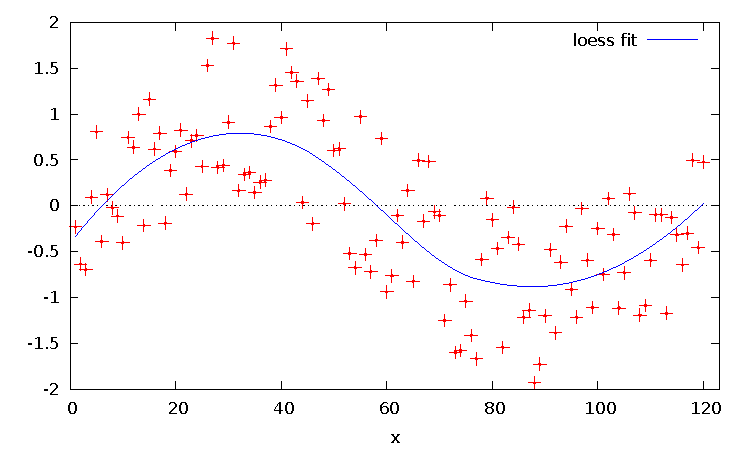
\includegraphics[scale=0.75]{figures/loess-sine}
  \caption{Loess: retrieving a sine wave}
  \label{fig:loess-sine}
\end{figure}

\section{The Nadaraya--Watson estimator}
\label{sec:nadarwat}

The Nadaraya--Watson nonparametric estimator \citep{nadaraya64,
  watson64} is an estimator for the conditional mean of a variable
$Y$, available in a sample of size $n$, for a given value of a
conditioning variable $X$, and is defined as
\[
  m(X) = \frac{ \sum_{j=1}^{n} y_j \cdot K_h(X - x_j)} {\sum_{j=1}^{n} K_h(X - x_j)}
\]
where $K_h(\cdot)$ is the so-called \emph{kernel function}, which is
usually some simple transform of a density function that depends on a
scalar called the \emph{bandwidth}. The one gretl uses is given
by
\[
  K_h(x) = \exp\left(-\frac{x^2}{2h}\right)
\]
for $|x| < \tau$ and zero otherwise. The scalar $\tau$ is used to
prevent numerical problems when the kernel function is evaluated too
far away from zero and is called the trim parameter.

\begin{script}[htbp]
  \caption{Nadaraya--Watson example}
  \label{scr:nadarwat-ex}
\begin{scode}
# Nonparametric regression example: husband's age on wife's age
open mroz87.gdt

# initial value for the bandwidth
scalar h = $nobs^(-0.2)
# three increasingly smooth estimates
series m0 = nadarwat(HA, WA, h)
series m1 = nadarwat(HA, WA, h * 5)
series m2 = nadarwat(HA, WA, h * 10)

# produce the graph
dataset sortby WA
gnuplot HA m0 m1 m2 WA --output=display --with-lines=m0,m1,m2
\end{scode}
%$
\end{script}

\begin{figure}[htbp]
  \centering
  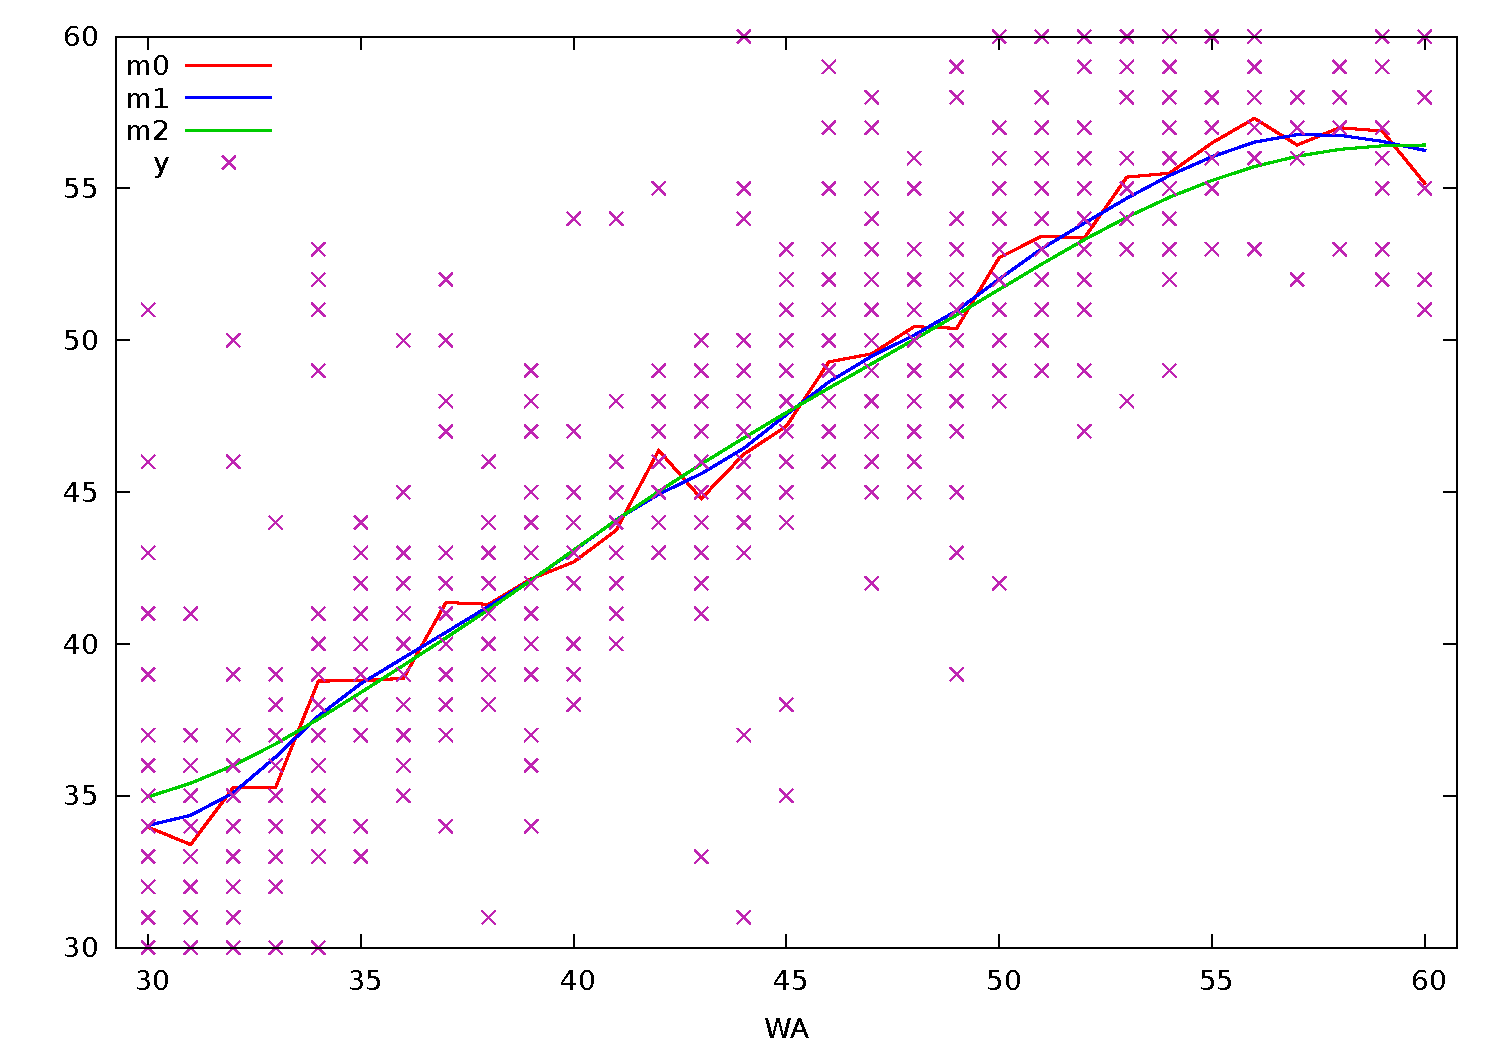
\includegraphics[scale=0.5]{figures/nadarwat-ex}
  \caption{Nadaraya--Watson example for several choices of the bandwidth parameter}
  \label{fig:nadarwat-ex}
\end{figure}

Listing~\ref{scr:nadarwat-ex} produces the graph shown in
Figure~\ref{fig:nadarwat-ex} (after some slight editing).

The choice of the bandwidth is up to the user: larger values of $h$
lead to a smoother $m(\cdot)$ function; smaller values make the
$m(\cdot)$ function follow the $y_i$ values more closely, so that the
function appears more ``jagged''. In fact, as $h \to \infty$, $m(x_i)
\to \bar{Y}$; on the contrary, if $h \to 0$, observations for which
$x_i \ne X$ are not taken into account at all when computing $m(X)$.

Also, the statistical properties of $m(\cdot)$ vary with $h$: its
variance can be shown to be decreasing in $h$, while its squared bias
is increasing in $h$.  It can be shown that choosing $h \sim n^{-1/5}$
minimizes the RMSE, so that value is customarily taken as a reference
point.

Note that the kernel function has its tails ``trimmed''. The scalar
$\tau$, which controls the level at which trimming occurs is set by
default at $4 \cdot h$; this setting, however, may be changed via the
\cmd{set} command. For example,
\begin{code}
  set nadarwat_trim 10
\end{code}
sets $\tau = 10 \cdot h$. This may at times produce more sensible
results in regions of $X$ with sparse support; however, you should be
aware that in those same cases machine precision (division by
numerical zero) may render your results spurious. The default is
relatively safe, but experimenting with larger values may be a sensible
strategy in some cases.

A common variant of the Nadaraya--Watson estimator is the so-called
``leave-one-out'' estimator: this is a variant of the estimator that
does not use the $i$-th observation for evaluating $m(x_i)$. This
makes the estimator more robust numerically and its usage is often
advised for inference purposes.  In formulae, the leave-one-out
estimator is
\[
m(x_i) = \frac{ \sum_{j \ne i} y_j \cdot K_h(x_i -
  x_j)} {\sum_{j \ne i} K_h(x_i - x_j)}
\]
In order to have gretl compute the leave-one-out estimator, just
reverse the sign of $h$: if we changed example \ref{scr:nadarwat-ex} by
substituting
\begin{code}
  scalar h = $nobs^(-0.2)
\end{code}
with
\begin{code}
  scalar h = -($nobs^(-0.2))
\end{code}
the rest of the example would have stayed unchanged, the only
difference being the usage of the leave-one-out estimator.

Although $X$ could be, in principle, any value, in the typical usage
of this estimator you want to compute $m(X)$ for $X$ equal to one or
more values actually observed in your sample, that is $m(x_i)$. If you
need a point estimate of $m(X)$ for some value of $X$ which is not
present among the valid observations of your dependent variable, you
may want to add some ``fake'' observations to your dataset in which
$y$ is missing and $x$ contains the values you want $m(x)$ evaluated
at. For example, the following script evaluates $m(x)$ at regular
intervals between -2.0 and 2.0:

\begin{code}
nulldata 120
set seed 120496

# first part of the sample: actual data
smpl 1 100
x = normal()
y = x^2 + sin(x) + normal()

# second part of the sample: fake x data
smpl 101 120
x = (obs-110) / 5

# compute the Nadaraya-Watson estimate
# with bandwidth equal to 0.4 (note that
# 100^(-0.2) = 0.398)
smpl full
m = nadarwat(y, x, 0.4)

# show m(x) for the fake x values only
smpl 101 120
print x m -o
\end{code}

and running it produces
\begin{code}
               x            m

101         -1.8     1.165934
102         -1.6     0.730221
103         -1.4     0.314705
104         -1.2     0.026057
105         -1.0    -0.131999
106         -0.8    -0.215445
107         -0.6    -0.269257
108         -0.4    -0.304451
109         -0.2    -0.306448
110          0.0    -0.238766
111          0.2    -0.038837
112          0.4     0.354660
113          0.6     0.908178
114          0.8     1.485178
115          1.0     2.000003
116          1.2     2.460100
117          1.4     2.905176
118          1.6     3.380874
119          1.8     3.927682
120          2.0     4.538364
\end{code}

%%% Local Variables: 
%%% mode: latex
%%% TeX-master: "gretl-guide"
%%% End: 
